%%%%%%%%%%%%%%%%%%%%%%%%%%%%%%%%%%%%%%%%%
% Beamer Presentation
% LaTeX Template
% Version 1.0 (10/11/12) 
%
% This template has been downloaded from:
% http://www.LaTeXTemplates.com
%
% License:
% CC BY-NC-SA 3.0 (http://creativecommons.org/licenses/by-nc-sa/3.0/)
%
%%%%%%%%%%%%%%%%%%%%%%%%%%%%%%%%%%%%%%%%%

%----------------------------------------------------------------------------------------
%	PACKAGES AND THEMES
%----------------------------------------------------------------------------------------

\documentclass{beamer}

\mode<presentation> {
%\mode<handouts> {
%\mode<article> {


% The Beamer class comes with a number of default slide themes
% which change the colors and layouts of slides. Below this is a list
% of all the themes, uncomment each in turn to see what they look like.


%\usetheme{default}
%\usetheme{AnnArbor}
%\usetheme{Antibes}
%\usetheme{Bergen}
%\usetheme{Berkeley}
%\usetheme{Berlin}
%\usetheme{Boadilla}
\usetheme{CambridgeUS}
%\usetheme{Copenhagen}
%\usetheme{Darmstadt}
%\usetheme{Dresden}
%\usetheme{Frankfurt}
%\usetheme{Goettingen}
%\usetheme{Hannover}
%\usetheme{Ilmenau}
%\usetheme{JuanLesPins}
%\usetheme{Luebeck}
%\usetheme{Madrid}
%\usetheme{Malmoe}
%\usetheme{Marburg}
%\usetheme{Montpellier}
%\usetheme{PaloAlto}
%\usetheme{Pittsburgh}
%\usetheme{Rochester}
%\usetheme{Singapore}
%\usetheme{Szeged}
%\usetheme{Warsaw}

% As well as themes, the Beamer class has a number of color themes
% for any slide theme. Uncomment each of these in turn to see how it
% changes the colors of your current slide theme.

%\usecolortheme{albatross}
\usecolortheme{beaver}
%\usecolortheme{beetle}
%\usecolortheme{crane}
%\usecolortheme{dolphin}
%\usecolortheme{dove}
%\usecolortheme{fly}
%\usecolortheme{lily}
%\usecolortheme{orchid}
%\usecolortheme{rose}
%\usecolortheme{seagull}
%\usecolortheme{seahorse}
%\usecolortheme{whale}
%\usecolortheme{wolverine}

%\setbeamertemplate{footline} % To remove the footer line in all slides uncomment this line
%\setbeamertemplate{footline}[page number] % To replace the footer line in all slides with a simple slide count uncomment this line

%\setbeamertemplate{navigation symbols}{} % To remove the navigation symbols from the bottom of all slides uncomment this line
}

\usepackage{graphicx} % Allows including images
\graphicspath{{../figures}}
\usepackage{booktabs} % Allows the use of \toprule, \midrule and \bottomrule in tables
\usepackage{amsmath, amssymb, amsthm, gensymb,mathrsfs}%,eufrak}
\usepackage{hyperref}
\usepackage{tabularx}
\usepackage{longtable}
\usepackage{makecell}
\usepackage{multicol}
\usepackage{physics}

\newcommand{\uvec}[1]{\textbf{#1}}

\newcounter{excounter}
%\renewcommand{\thefpcounter}{\thechapter.\arabic{fpcounter}}
%\renewcommand{\thefpcounter}{\thesection.\arabic{fpcounter}}
\renewcommand{\theexcounter}{\arabic{excounter}}

\newtheorem{teorema}{Teorema}[section]
\newtheorem{definicio}{Definició}[section]

\usepackage[lastexercise]{exercise}

\graphicspath{{../figures}}

%----------------------------------------------------------------------------------------
%	 TITLE PAGE
%----------------------------------------------------------------------------------------

\title[SVM]{Support Vector Machine} % The short title appears at the bottom of every slide, the full title is only on the title page

\author{Jordi Villà i Freixa} % Your name
\institute[FCTE] % Your institution as it will appear on the bottom of every slide, may be shorthand to save space
{
Universitat de Vic - Universitat Central de Catalunya \\
Study Abroad\\ % Your institution for the title page
\medskip
\textit{jordi.villa@uvic.cat} % Your email address
}
%\date{\today} % Date, can be changed to a custom date
\date{course 2023-2024}
\logo{
\includegraphics[width=.1\textwidth]{FCTE}}

\newcommand\MyBox[2]{
  \fbox{\lower0.75cm
    \vbox to 1.7cm{\vfil
      \hbox to 1.7cm{\hfil\parbox{1.4cm}{#1\\#2}\hfil}
      \vfil}%
  }%
}

\begin{document}

\begin{frame}
\titlepage % Print the title page as the first slide
\end{frame}

\begin{frame}
\frametitle{Índex} % Table of contents slide, comment this block out to remove it
\tableofcontents % Throughout your presentation, if you choose to use \section{} and \subsection{} commands, these will automatically be printed on this slide as an overview of your presentation
\end{frame}

%----------------------------------------------------------------------------------------
%	PRESENTATION SLIDES
%----------------------------------------------------------------------------------------


\section{Introduction}

\begin{frame}{Support-vector machine and kermel functions}
  \begin{figure}
    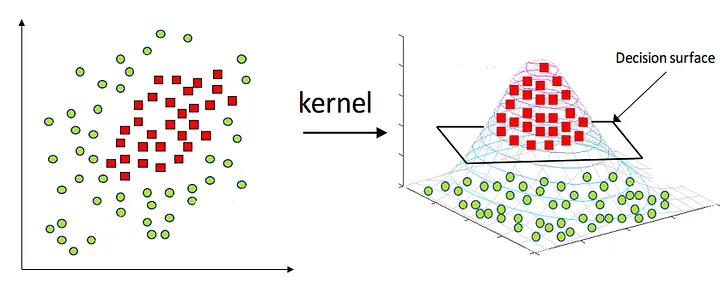
\includegraphics[width=0.7\textwidth]{SVM2}
  \end{figure}
\end{frame}


\begin{frame}
  Support-vector machines (SVMs) are a set of algorithms of supervised learning developed by Vladimir Vapnik and his team at the AT\&T Bell labs.
  \\[10pt]
  Let us take a labelled dataset with two classes or categories. Our goal is to predict the category of a new data point. 
  Intuitively, an SVM is a model that represents the points of a dataset in space, separating the two classes into two subespaces that are as large as possible by means of a hyperplane that depends on the position of the closest points between the two classes (the support vector).
\end{frame}

\begin{frame}{Example in 2 dimensions}
  \begin{columns}
    \begin{column}{0.4\textwidth}
   The SVM algorithm looks for a hyperplane, in this case a straight line, that separates the two data categories. But which? The one that provides a larger margin between the elements of the two categories.
    \end{column}
  \begin{column}{0.4\textwidth}
  \begin{figure}
    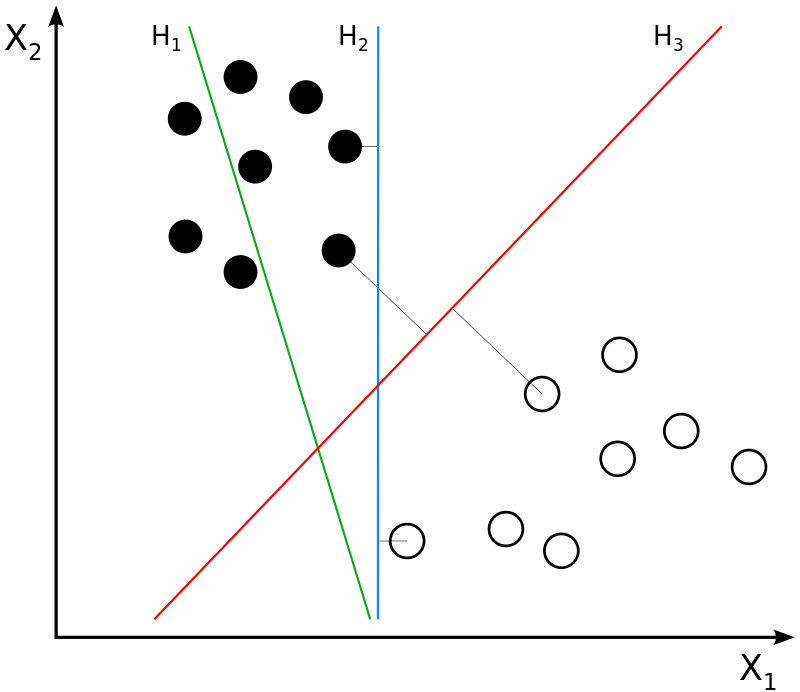
\includegraphics[width=\textwidth]{Svm_4}
  \end{figure}
\end{column}
\end{columns}
\end{frame}


\begin{frame}
  {\bf Support vectors} are the data points, which are closest to the hyperplane. These points will define the separating line better by calculating margins. These points are more relevant to the construction of the classifier.
  \\[10pt]
  A {\bf hyperplane} is a decision plane which separates between a set of objects having different class memberships. If we have $p$-dimensional space, a hyperplane is a flat subspace with dimension $p-1$. In $\mathbb{R}^3$, the hyperplane is a line $\beta_0+\beta_1 X_1+\beta_2 X_2=0$. In $\mathbb{R}^p$,  
  \begin{equation}
    \beta_0+\beta_1 X_1+\beta_2 X_2 + \cdots + \beta_p X_p=0 \label{Eq:hyperp}
  \end{equation}
  \\[10pt]
  A {\bf margin} is a gap between the two lines on the closest class points. This is calculated as the perpendicular distance from the line to support vectors or closest points. If the margin is larger in between the classes, then it is considered a good margin, a smaller margin is a bad margin.
\end{frame}

\begin{frame}{Hyperplane}
  Following the definition of the hyperplane, if a point $X = (X_1,X_2,\ldots,X_p)^T$ in $\mathbb{R}^p$ satisfies \ref{Eq:hyperp}, then X lies on the hyperplane.  Now, suppose that X does not satisfy (9.2); rather,
  \begin{eqnarray*}
    \beta_0+\beta_1 X_1+\beta_2 X_2 + \cdots + \beta_p X_p&>&0\\ 
    \beta_0+\beta_1 X_1+\beta_2 X_2 + \cdots + \beta_p X_p&<&0 
  \end{eqnarray*}
  then X lies above or below the hyperplane.  One can easily determine on which side of the hyperplane a point lies by simply calculating the sign of the left hand side of \ref{Eq:hyperp}. 
\end{frame}
  
  \begin{frame}{Hyperplane}
    \begin{figure}
      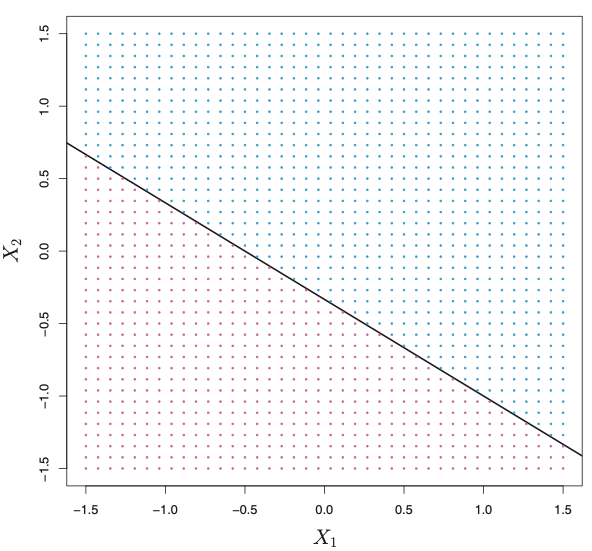
\includegraphics[width=0.5\textwidth]{hyperplane2D}
      \caption{Hyperplane in 2D $1 + 2X_1 + 3X_2 = 0$. The blue and purple regions show points above and below the hyperplane (adapted from \cite{sohil_introduction_2022}).}
    \end{figure}
  \end{frame}

\begin{frame}{Hyperplane}
  \begin{figure}
    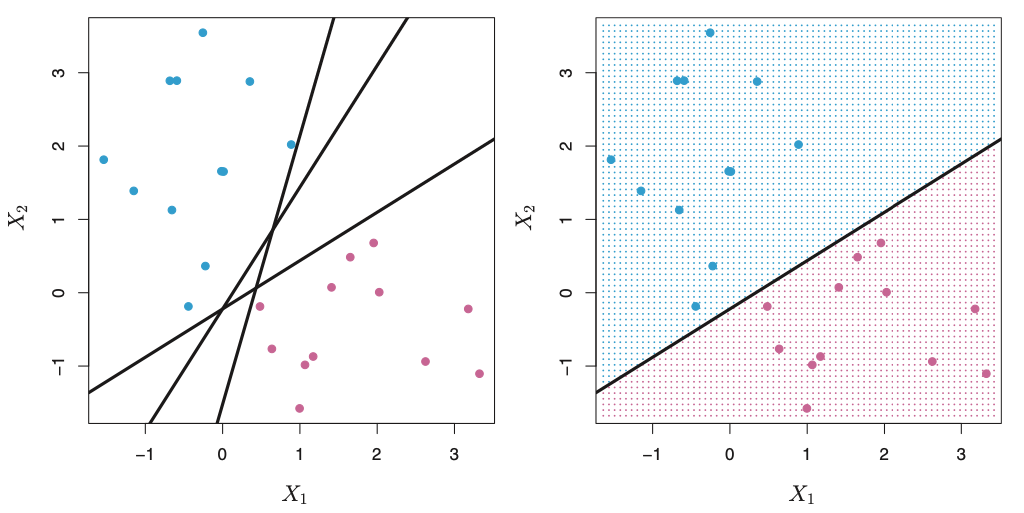
\includegraphics[width=0.7\textwidth]{hyperplanes}
    \caption{If our data can be perfectly separated using a hyperplane, then there will in fact exist an infinite number of such hyperplanes. \cite{sohil_introduction_2022}.}
  \end{figure}
\end{frame}

\section{Maximal MArgin Classifier}

\begin{frame}{Maximal Margin Classifier}

  In order to construct a classifier based upon a separating hyperplane, we must have a reasonable way to decide which of the infinite possible separating hyperplanes to use.
  \\[10pt]
  A natural choice is the maximal margin hyperplane (also known as the optimal separating hyperplane), which is the separating hyperplane that is farthest from the training observations.\cite{sohil_introduction_2022}
\end{frame}


\begin{frame}{Support vectors}
  \begin{figure}
    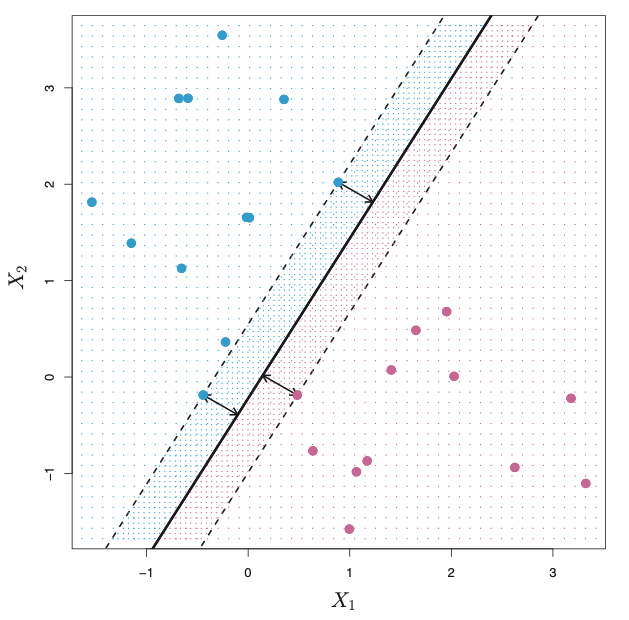
\includegraphics[width=0.5\textwidth]{supportvectors}
    \caption{Support vectors \cite{sohil_introduction_2022}.}
  \end{figure}
\end{frame}

\begin{frame}{Maximal Margin Classifier}
  \begin{itemize}
  \item The maximal margin hyperplane is the separating hyperplane for which the margin is largest.
  \item We hope that a classifier that has a large margin on the training data will also have a large margin on the test data, and hence will classify the test observations correctly. 
  \item The maximal margin hyperplane represents the mid-line of the widest “slab” that we can insert between the two classes.
  \item Leads to overfitting when $p$ is large. 
  \item Very sensitive to the training data. It will perform perfectly on the training data set, but maybe poorly on the unseen data. 
  Though it is elegant and simple, this classifier unfortunately cannot be applied to most data sets, since it requires that the classes be separable by a {\bf linear boundary}. 
  \end{itemize}
\end{frame}

\begin{frame}{Building a MMC}
  \begin{equation*}
    \begin{aligned}
      \text{maximize } \quad & M=M(\beta_0,\beta_1,\ldots,\beta_p) \\
      \text{subject to }\quad &
      \begin{array}{l}
        \sum_{j=1}^p \beta_j^2 =1 \\
        y_i(\beta_0+\beta_1x_{i1}+\cdots+\beta_p x_{ip})\geq M \; \forall \; i=1,\ldots,n
      \end{array}
    \end{aligned}
  \end{equation*}
\end{frame}

\section{Support Vector Classifier}


\begin{frame}{Sensitivity of the hyperplane}
  \begin{figure}
    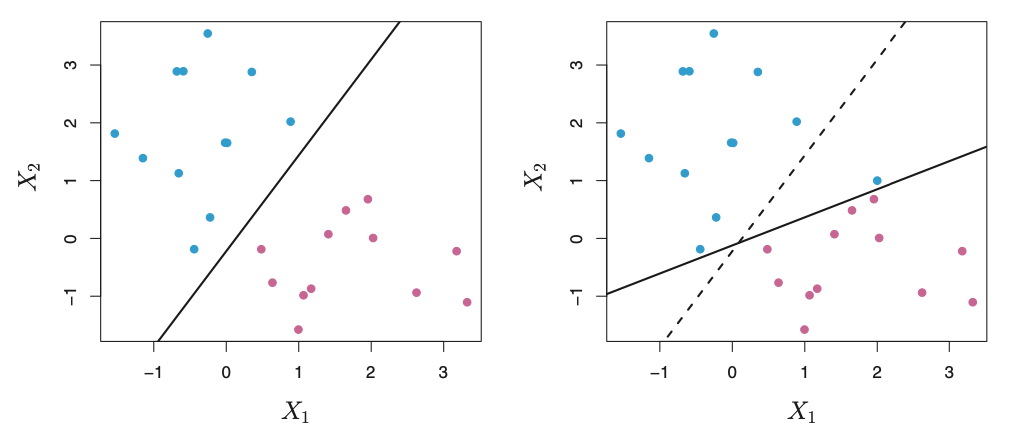
\includegraphics[width=0.7\textwidth]{sensitivityhyperplane}
    \caption{The addition of a single point leads to a dramatic shift in the maximal margin hyperplane shown as a solid line\cite{sohil_introduction_2022}.}
  \end{figure}
\end{frame}

\begin{frame}{Soft Margin Classifier}
  \begin{itemize}
  \item  We need a classifier with greater robustness to individual observations, and better classification of most of the training observations.
  The generalization of the maximal margin classifier to the non-separable case is known as the support vector classifier or soft margin classifier.
  \item It is {\bf still linear} a modification of the Maximal-Margin Classifier to relax the margin to handle noisy class boundaries in real data.
  \item It allows certain points to be deliberately misclassified. By doing this, it is able to classify most of the points correctly in the unseen data and is also more robust. 
  \item An observation can be not only on the wrong side of the margin, but also on the wrong side of the hyperplane. Observations on the wrong side of the hyperplane correspond to training observations that are misclassified by the support vector classifier.
  \end{itemize}
\end{frame}

\begin{frame}
  \begin{figure}
    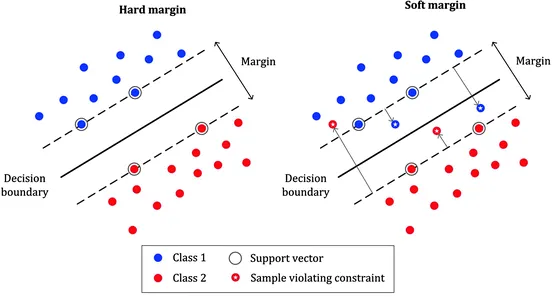
\includegraphics[width=0.9\textwidth]{SVM3}
  \end{figure}
\end{frame}

\begin{frame}{Building a SVC}
  \begin{equation*}
    \begin{aligned}
      \text{maximize } \quad & M=M(\beta_0,\beta_1,\ldots,\beta_p,\varepsilon_1,\ldots,\varepsilon_n) \\
      \text{subject to }\quad &
      \begin{array}{l}
        \sum_{j=1}^p \beta_j^2 =1 \\
        y_i(\beta_0+\beta_1x_{i1}+\cdots+\beta_p x_{ip})\geq M(1-\varepsilon_i) \; \forall \; i=1,\ldots,n\\
        \varepsilon_i\geq 0, \; \sim_{i=1}^n\leq C
      \end{array}
    \end{aligned}
  \end{equation*}
\end{frame}

\begin{frame}{Slack variable $\varepsilon_i$}
  \begin{itemize}
    \item Slack variables are introduced to allow certain constraints to be violated. That is, certain training points will be allowed to be within the margin:
    \begin{itemize}
      \item If $\varepsilon_i = 0$ then the ith slack variable observation is on the correct side of the margin
      \item If $\varepsilon_i > 0$ then the ith observation is on the wrong side of the margin (it has violated the margin)
      \item If $\varepsilon_i > 1$ then it is on the wrong side of the hyperplane.
    \end{itemize}
    \item We want the number of points within the margin to be as small as possible, and of course we want their penetration of the margin to be as small as possible.
  \end{itemize}
\end{frame}


\begin{frame}
  \begin{figure}
    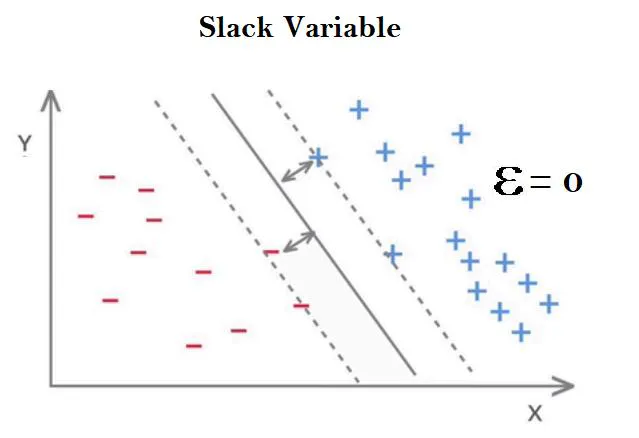
\includegraphics[width=0.7\textwidth]{Slack}
  \end{figure}
\end{frame}

\begin{frame}
  But if you draw a Support Vector Classifier in such a way that it only violates the margin, i.e. $0< \varepsilon < 1$, the observations classify correctly as shown in figure below.
  \begin{figure}
    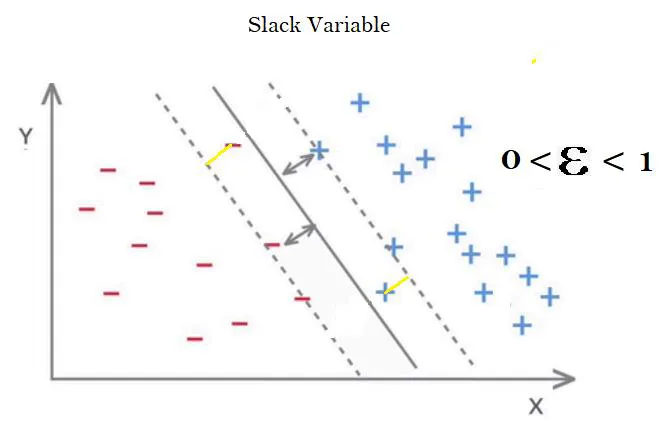
\includegraphics[width=0.7\textwidth]{Slack2}
  \end{figure}
\end{frame}

\begin{frame}
  If the data points violate the hyperplane, i.e. $\varepsilon(ϵ) > 1$, then the observation is on the wrong side of the hyperplane.

  \begin{figure}
    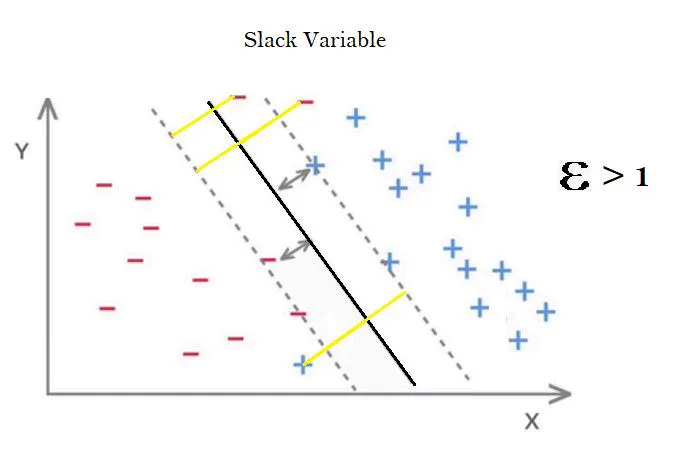
\includegraphics[width=0.7\textwidth]{Slack3}
  \end{figure}
\end{frame}

\begin{frame}{Cost of missclassification}
  \begin{itemize}
    \item Cost of misclassification, $C$, is greater than or equal to the summation of all the epsilons of each data point.
    \item When $C$ is large, you allow a larger number of data points to be misclassified or to violate the margin.
    \item When $C$ is small, the margin is narrow and there are few misclassifications.
  \end{itemize}
\end{frame}

\section{Support vector machines}

\begin{frame}{Non-linear boundaries}
  \begin{figure}
    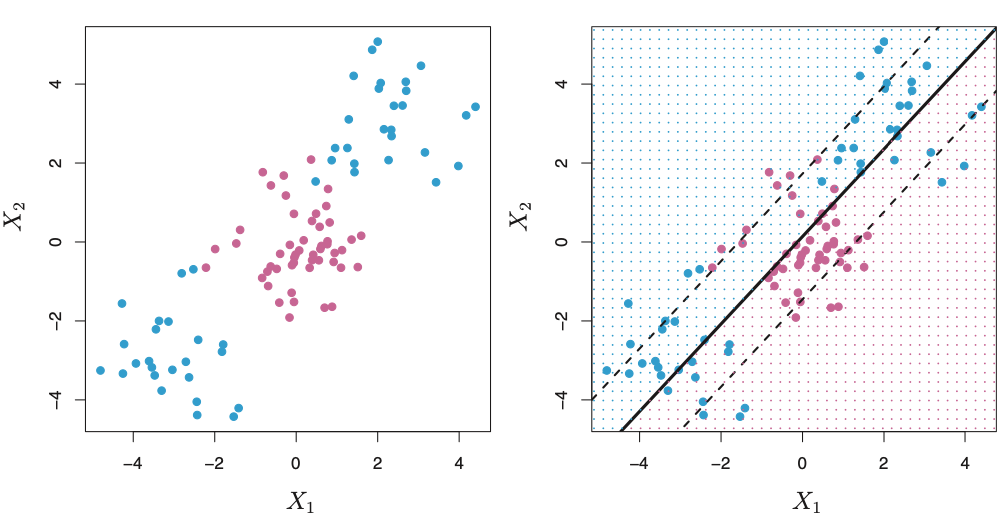
\includegraphics[width=0.7\textwidth]{nonlinearSVC}
    \caption{Left: The observations fall into two classes, with a non-linear boundary between them. Right: The support vector classifier seeks a linear bound- ary, and consequently performs very poorly\cite{sohil_introduction_2022}.}
  \end{figure}
\end{frame}

\begin{frame}{SVC with quadratic boundaries. Enlarging the feature space}
  \begin{equation*}
    \begin{aligned}
      \text{maximize } \quad & M=M(\beta_0,\beta_{11},\beta_{12}\ldots,\beta_{p1},\beta_{p2},\varepsilon_1,\ldots,\varepsilon_n) \\
      \text{subject to }\quad &
      \begin{array}{l}
        \sum_{j=1}^p \sum_{k=1}^2 \beta_{jk}^2 =1 \\
        y_i(\beta_0+\sum_{j=1}^{p}\beta_{j1}x_{ij}+\sum_{j=1}^{p} \beta_{j2} x_{ij}^2)\geq M(1-\varepsilon_i) \; \forall \; i=1,\ldots,n\\
        \varepsilon_i\geq 0, \; \sim_{i=1}^n\leq C
      \end{array}
    \end{aligned}
  \end{equation*}
\end{frame}

\begin{frame}{Kernels}
  \begin{itemize}
    \item We may want to enlarge our feature space support vector machine kernel in order to accommodate a non-linear boundary between the classes.
    \item The kernel approach is an efficient computational approach for enacting this idea.
    \item The function of kernel is to take data as input and transform it into the required form. 
    \item Different SVM algorithms use different types of kernel functions. These functions can be linear, nonlinear, polynomial, radial basis function (RBF), and sigmoid.
  \end{itemize}
\end{frame}

\begin{frame}{SVC includes just inner products of the observations}
  It can be shown that\cite{sohil_introduction_2022}
  \begin{itemize}
    \item The linear support vector classifier, for $n$ training observations, can be represented as
    \[
      f(x)=\beta_0 + \sum_{i=1}^n \alpha_i <x,x_i>
    \]
    \item To estimate the parameters $\alpha_i$ we just need the inner products of the support vectors 
    \[
      f(x)=\beta_0 + \sum_{i\in S}^n \alpha_i <x,x_i>
    \]
  \end{itemize}
  What if we could substitute the collection of inner products by other functions that would help us expanding features in an efficient way? This is using kernels in SVM.
\end{frame}

\begin{frame}{Mapping data to higher dimensions}
  \begin{figure}
    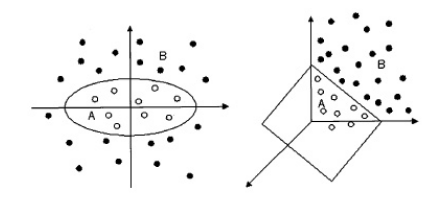
\includegraphics[width=0.7\textwidth]{mappingSVM}
    \caption{Mapping of non-linear separable training data from $\mathbb{R}^2$ into $\mathbb{R}^3$ \cite{hofmann_support_2006}.}
  \end{figure}
\end{frame}

\begin{frame}
\begin{itemize} 
  \item As feature transformation results in large number of features, it makes the modelling (i.e. the learning process) computationally expensive. The use of kernel resolves this issue. A kernel is a function that quantifies the similarity of two observations. In case of the linear kernel, it provides the SVC:
  \[K(X_i,X_i')=\sum_{j=1}^p x_{ij}x_{i'j}\]
  \item To find a best fit model, the learning algorithm only needs the inner products of the observations. 
  \item Kernel Function generally transforms the training set of data so that a non-linear decision surface is able to transformed to a linear equation in a higher number of dimension spaces. 
  \item Basically, It returns the inner product between two points in a standard feature dimension.
\end{itemize}
\end{frame}

\begin{frame}{Popular kernels}
  \begin{itemize}
    \item The linear kernel.
    \item The polynomial kernel.
    \item The radial basis function (RBF) kernel. It is capable of creating elliptical (i.e. enclosed) decision boundaries.
    \item The sigmoid kernel.
  \end{itemize}
  \begin{figure}
    \includegraphics[width=0.7\textwidth]{kernelsSVM}
  \end{figure}
\end{frame}

\section{Bibliography}
\bibliographystyle{unsrt}
\bibliography{DataSciencewithPython}
\end{document}